\chapter{Description of the Methods}
\label{chap:description}
In this chapter, the two methods \cite{Lin04radiometriccalibration} and \cite{ng_cvpr07} treated in this thesis are presented. $r(x,y)$ and $R(x,y)$ are used respectively for image irradiance and image intensity, where $x$ and $y$ specify the pixel position in the coordinate frame of the image. The CRF is denoted either by $r = f(R)$ or by $R = g(r)$ in case of the inverse CRF.

Both papers share the assumptions, that the CRF of a camera is equal for \emph{every} image pixel and that the red, green and blue colors are accurately measured for each pixel (see \autoref{chap:crf}).

The implementations are written in \emph{C++} and based on the \emph{OpenCV} library \cite{opencv_library}, version 2.1 from April 2010.




\clearpage

%%%%%%%%%%%%%%%%%%%%%%
% RadCal
%%%%%%%%%%%%%%%%%%%%%%

\section{Radiometric Calibration from a Single Image}
\label{sec:radcal}
This method published by Stephen Lin et \hbox{al.} in 2004 \cite{Lin04radiometriccalibration} is among the earliest, where the automatic determination of the CRF from only a single arbitrary image is addressed. Like many other approaches from various authors, their method makes use of the 201 real world CRFs from the DoRF database compiled by M.D. Grossberg and S.K. Nayar and presented in their 2004 IEEE article \cite{CAVE_0091}.

``Radiometric Calibration from a Single Image'' requires image specific data acquisition by finding small patches in the image, which provide the data for a derivation of the applied CRF. If not sufficiently many patches are found, the method will fail either completely or lead to highly unstable estimates, because then the coverage of the $R$-space is only sparse. To overcome this, it is also possible to use more than only one image of the specific camera -- if available -- to obtain a higher amount of data.

\vspace{1cm}

\subsection{Theoretical Foundation}
\label{subsec:radcaltheory}
%This approach is based on the nonlinearity of edge color distributions.

\subsubsection{Nonlinearity of Edge Colors}
\label{subsubsec:nonlinearityofedgecolors}
Let $P$ be an image patch that contains two distinct regions separated by an edge, each having different but at most uniform colors $C_1$ and $C_2$. Due to the limited spatial resolution of a CCD sensor (visualized through the grid in \autoref{fig:illustrationedgenonlinearity}), the color of each edge pixel results in a linear combination of the two region colors $C_1$ and $C_2$. Hence, the colors of the edge pixels $C_{\text{edge}}$ lie on a line between $C_1$ and $C_2$ in RGB-space.
\begin{equation}
	C_{\text{edge}} = \alpha \cdot C_1 + (1 - \alpha) \cdot C_2 \enspace , 
	\label{eq:linearcombination}
\end{equation}
where $\alpha \in [0;1]$ denotes the ratio of the area in the pixel which is covered by $C_1$ to the total area of the pixel in scene radiance.

For an illustration of this interpolation see \autoref{fig:illustrationedgenonlinearity} on page \pageref{fig:illustrationedgenonlinearity}. The first image, \autoref{subfig:radiance}, shows an exemplary part of a scene (scene radiance) containing a clear edge and thus two regions of different color. In \autoref{subfig:radiancewitharray} the latter is overlayed by a grid, representing the discrete CCD sensor array. Note that the edge divides four of the array cells into two distinct regions each. \autoref{subfig:irradiance} shows the image irradiance after the linear interpolation inside the cells containing the edges as described in \autoref{eq:linearcombination}. The result of applying a basic CRF, a gamma curve with $\gamma = 0.4$, is presented in \autoref{subfig:intensity}.

\begin{figure}[tbp]
  \centering
  \subfigure[Radiance]{
    \label{subfig:radiance}
    
\includegraphics[width=0.22\textwidth]{images/patch.png} 
  }
  \subfigure[Radiance with grid]{
    \label{subfig:radiancewitharray}
    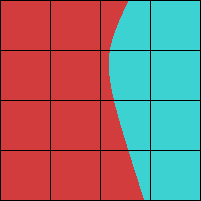
\includegraphics[width=0.22\textwidth]{images/patch_with_array.png} 
  }
  \subfigure[Irradiance]{
    \label{subfig:irradiance}
    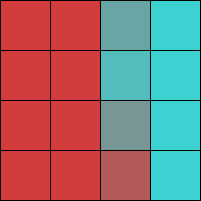
\includegraphics[width=0.22\textwidth]{images/patch_with_array_irradiance.png} 
  }
  \subfigure[Intensity]{
    \label{subfig:intensity}
    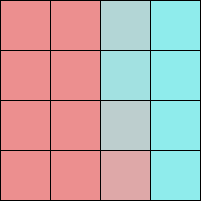
\includegraphics[width=0.22\textwidth]{images/patch_with_array_gamma04.png} 
  }
  \caption[Illustration of edge pixel distributions]{Illustration of edge pixel distributions.}
  \label{fig:illustrationedgenonlinearity}
\end{figure}

But \autoref{eq:linearcombination} only holds in the domain of \emph{image irradiance}. After the mapping from image irradiance to image intensity -- regarding the nonlinearity of the CRF -- the edge pixel colors are not located on the line between the two region colors anymore (see the plot in \autoref{fig:gammavsnogamma}). This fact is exploited to estimate the camera response function. The points on the longer one of the two lines in \autoref{fig:gammavsnogamma} depict the colors in \autoref{subfig:irradiance} and the other points the colors after the CRF transformation as in \autoref{subfig:intensity}. The lines are spanned by the region colors. This illustrates the assumption that the linear distribution changed to a nonlinear one by applying the CRF. 

\begin{figure}[bth]
	\centering
	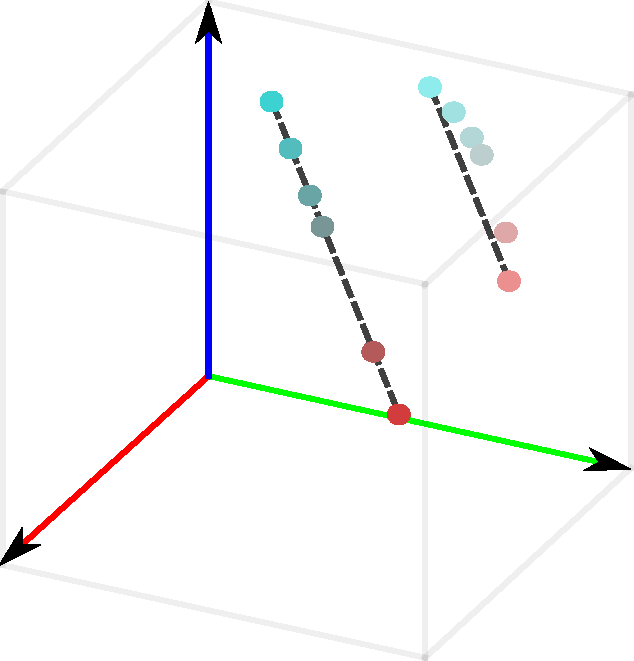
\includegraphics[width=0.4\textwidth]{plots/rgb_cube.pdf} 
  \caption[Illustration of intensity nonlinearities after gamma transformation (RGB-cube)]{Illustration of intensity nonlinearities after gamma transformation (RGB-cube).}  
  \label{fig:gammavsnogamma}
\end{figure}


\clearpage

\subsubsection{Transformation to Linear Distributions}
\label{subsubsec:transformationtolineardistributions}
Now, if a certain function $h$ can be found, which -- for every edge patch in the image -- maps the edge colors back onto the line between $h(C_1)$ and $h(C_2)$, this function is the inverse CRF $g = h$, or at least a sufficiently good approximation. Thus, for all edge patches $\omega$ in the set of edge patches $\Omega$, the distance $d(g;\omega_i)$ of the edge color $g(C_{\text{edge}})$ to the line spanned by the two region colors has to be zero:
\begin{equation}
	d(g;\omega) = \frac{\left|\left[g(C_1)-g(C_2)\right] \times \left[g(C_1)-g(C_{\text{edge}})\right] \right|} {\left|g(C_1)-g(C_2)\right|} = 0 \enspace ,
	\label{eq:distancepointtoline}
\end{equation}
where $\left|\cdot\right|$ indicates the absolute value and $\times$ denotes the cross product between two vectors. Note that the colors $C_1$, $C_2$ and $C_{\text{edge}}$ are RGB-colors and therefore three-dimensional vectors. 
The accumulated distance for all $\omega \in \Omega$ will be referred to as $D(g;\Omega) = \sum_{\omega \in \Omega}{d(g;\omega)}$ in the following. The \emph{likelihood function} $p(\Omega|g)$ is computed by an exponential distribution
\begin{equation}
	p(\Omega|g) = \frac{1}{Z} \cdot \exp({-\lambda \cdot D(g;\Omega)}) \enspace ,
	\label{eq:likelihoodfunction}
\end{equation}
where $Z$ is a normalization constant and $\lambda$ an important weighting factor, which will be examined in \autoref{chap:evaluation}.

Hence, the inverse response function and thus the CRF could be estimated by minimizing \autoref{eq:distancepointtoline}, but the accuracy can be enhanced by incorporating prior knowledge on (inverse) CRFs based on DoRF. Problems appearing when only sparse $R$-coverage is available are bypassed by using this prior knowledge. A PCA representation as presented in \cite{CAVE_0091} is chosen to model the CRFs. Additionally, $g$ can be computed straight forward
\begin{equation}
	g = g_{\text{mean}} + \vec{c} \cdot H \enspace .
	\label{eq:crfconcisedescriptorPCA}
\end{equation}
$g_{\text{mean}}$ is the mean inverse response curve over all inverted curves in DoRF, $\vec{c}$ is a coefficient vector in $\mathbb{R}^{\nu}$, $\nu$ is the number of used eigenvectors (obtained from the PCA) and $H$ is a matrix containing these eigenvectors. If we want $g$ to be defined as a vector containing the inverse CRF for all three channels, then all the variables except $H$ just get expanded, \hbox{i.e.} $\vec{c}$ is now a coefficient vector in $\mathbb{R}^{3 \times \nu}$ and so on.


\clearpage

\subsubsection{Prior Model}
\label{subsubsec:priormodel}
The prior model is formed as a Gaussian mixture model (GMM)
\begin{equation}
	p(g) = \sum\limits_{i=1}^\kappa \alpha_i \cdot \mathcal{N}(g; \mu_i, \Sigma_i) \enspace ,
	\label{eq:priormodel}
\end{equation}
where $g$ is the $\nu$-dimensional PCA representation of a particular inverse CRF, $\kappa$ the number of Gaussian kernels, $\alpha$ a weighting factor and $\mathcal{N}$ the multivariate normal distribution with $\mu$ as the mean vector and $\Sigma$ as the covariance matrix. The Gaussian mixture model and thus the mentioned parameters are obtained using the EM algorithm trained with the PCA representations of the 201 inverse CRFs extracted from DoRF. Note that the prior model fits only to an inverse CRF for a single color channel, so it has to be computed three times for the three channels in RGB images and combined afterwards. 


\clearpage

\subsection{The Algorithm}
\label{subsec:radcalalgo}
For an overview of the algorithm see the flow chart in \autoref{fig:radcaloverview} on page \pageref{fig:radcaloverview}.

\begin{figure}[htbp]
	\centering
	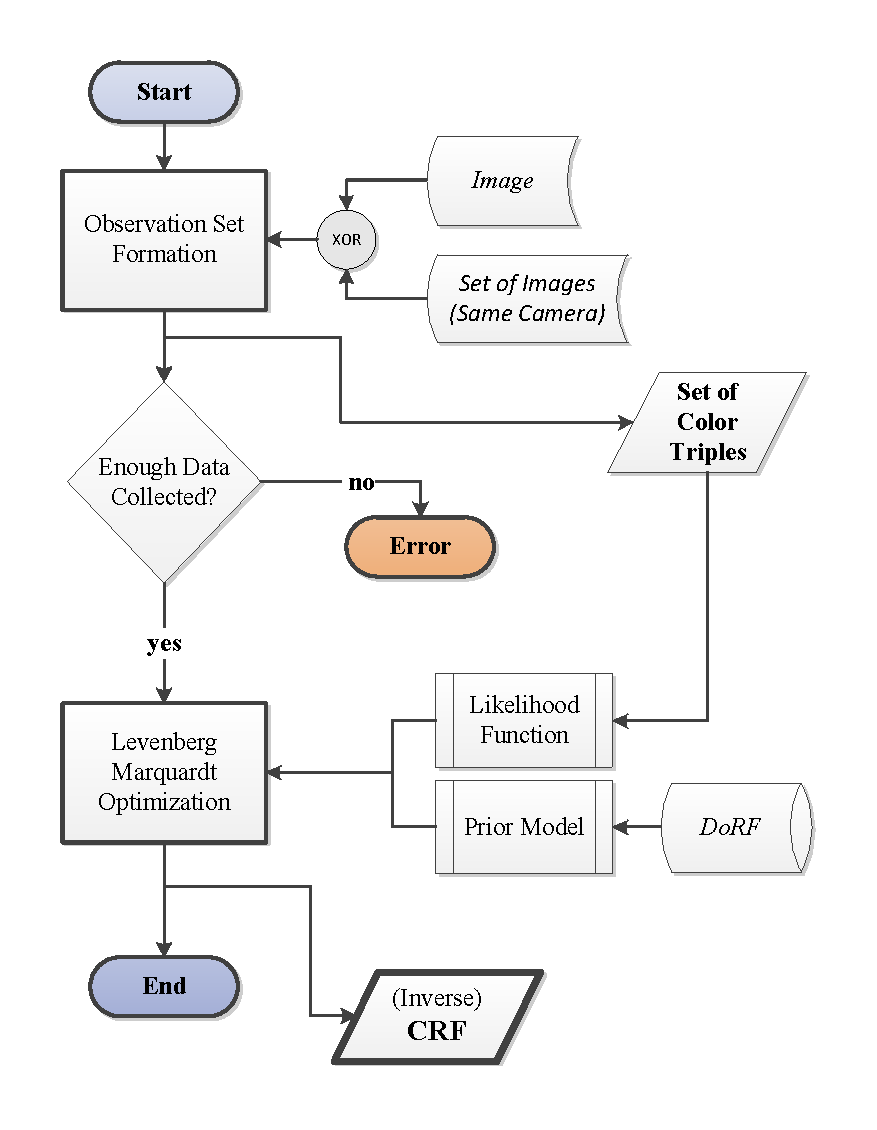
\includegraphics[width=0.9\textwidth]{images/radcal_overview.pdf}
	\caption[Flow chart (Radiometric Calibration)]{Flow chart of the algorithm. All important steps are presented in chronological order. Datasets and databases as well as the input and output of the algorithm are shown on the right.}
	\label{fig:radcaloverview}
\end{figure}

\subsubsection{Observation Set Formation}
\label{subsubsec:osf}
At first, image specific data is collected by analyzing either a single RGB image or sequentially a set of RGB images from the same camera with fixed settings. The method is based on \emph{edge} color distributions, so for locating potentially useful patches in the image, an edge image is created from the original image using the Canny operator \cite{canny1987computational}. The algorithm looks for patches of a certain fixed size $W \times H$ which are divided by an edge into exactly two regions of similar size. Like the choice of the author of this method, in this thesis the patches are squared, \hbox{i.e.} $W = H$, and unless differently stated, $W = H = 15$ pixels. As a candidate for the observation set $\Omega$, the considered patch has to meet the following conditions:
\begin{itemize}
	\item there is only one single, continuous edge path inside the patch,
	\item the color variance inside a region has to be below a specific threshold $\epsilon_\text{max}$,
	\item there has to be a minimum distance $\epsilon_\text{min}$ between the two region colors $C_1$ and $C_2$ and
	\item there are no spatially overlapping patches inside the observation set.
\end{itemize}
\begin{figure}
	\centering
	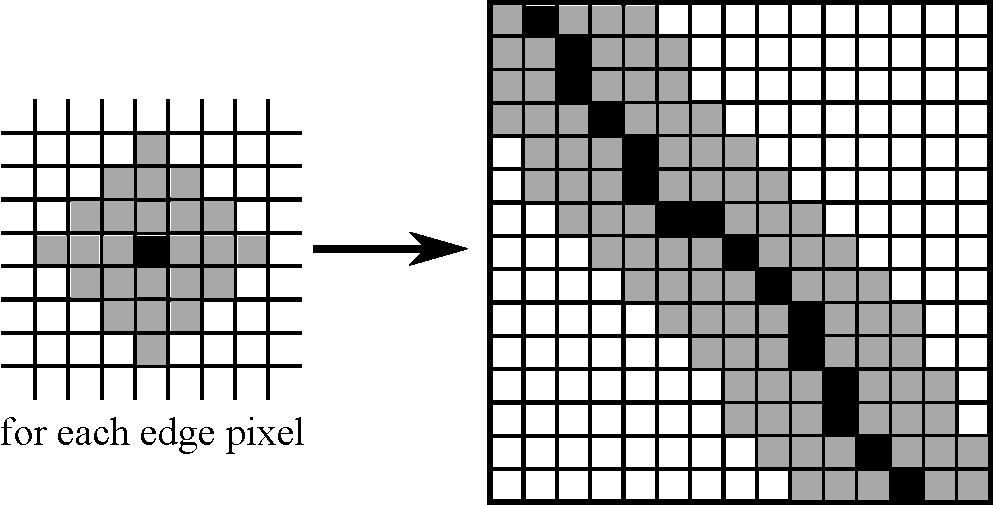
\includegraphics[width=0.5\linewidth]{images/dilation_illustration.pdf}
	\caption[Illustration of edge path dilation]{Illustration of edge path dilation. The size of the examined patch (right figure) is $15 \times 15$ pixels. Each cell in the array depicts one pixel. The edge path is given by the edge pixels (black). The dilation pixels are gray. The maximum distance from the dilation pixels to the edge path is set to 3 pixels. An example for the dilation for a single edge pixel is shown on the left.}
	\label{fig:dilationillustration}
\end{figure}
Due to the usually smooth transition from $C_1$ to $C_2$ over the edge path, the path is dilated by a few pixels, dependent on the chosen patch size $W \times H$. For patches of size $15 \times 15$ pixels, the maximum distance of each dilation pixel to the edge path has been experimentally set to 3 (for an illustration see \autoref{fig:dilationillustration}). 

Completely uniform region colors are usually very rare. Even if there is such a perfect region in scene radiance, the output of the CCD sensor is typically noisy. Hence, the finally used measurements for the region colors $C_1$ and $C_2$ are obtained by computing the mean colors inside the respective region, without considering the \emph{dilation pixels}. For each patch, several $C_{\text{edge}}$ values are available, depending on the amount of edge pixels -- or in other words -- on the length of the edge path. So more than just one \emph{edge color triple} ($C_1$, $C_2$ and $C_{\text{edge}}$) is generated for every patch by randomly choosing five of the colors on the edge path. After examining all $W \times H$ sized patches in the image or in the set of images, the data acquisition step is completed. Hence, the entire set of edge color triples $\Omega$ is compiled. A sample result of this \emph{observation set formation} is shown in \autoref{fig:patchselection} on page \pageref{fig:patchselection}. 

\begin{figure}[p]
  \centering
  \subfigure[Original image]{
    \label{subfig:patchimageorig}
    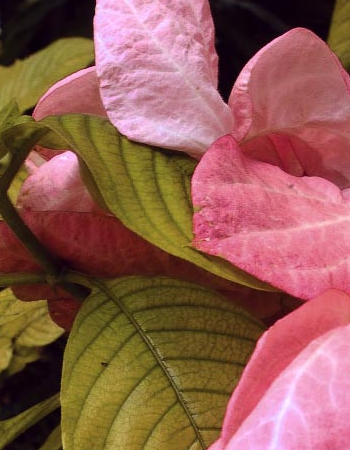
\includegraphics[width=0.45\textwidth]{images/image_for_patches_orig.png} 
  }
  \subfigure[Edge image with selected patches]{
    \label{subfig:patchimageedges}
    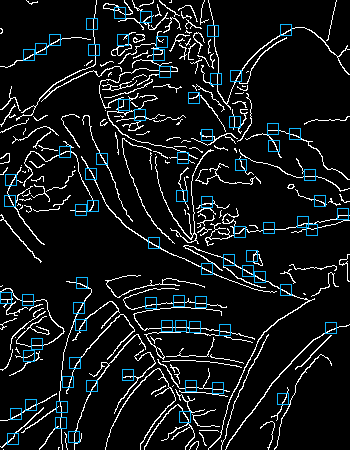
\includegraphics[width=0.45\textwidth]{images/image_for_patches_edge.png} 
  }
  \subfigure[Sample patch 1]{
    \label{subfig:samplepatch1}
    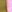
\includegraphics[width=0.22\textwidth]{images/patches/patch44-100.png} 
  }
  \subfigure[Sample patch 2]{
    \label{subfig:samplepatch2}
    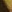
\includegraphics[width=0.22\textwidth]{images/patches/patch195-16.png} 
  }
  \subfigure[Sample patch 3]{
    \label{subfig:samplepatch3}
    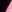
\includegraphics[width=0.22\textwidth]{images/patches/patch70-242.png}  
  }
  \subfigure[Sample patch 4]{
    \label{subfig:samplepatch4}
    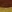
\includegraphics[width=0.22\textwidth]{images/patches/patch294-34.png}  
  }
  \caption[Selection of appropriate edge patches]{Selection of appropriate edge patches with patch size $12 \times 12$ pixels. The top left image is the original image. On the top right side, the Canny detected edge image is shown. The blue rectangles frame all selected patches. \autoref{subfig:samplepatch1} to \autoref{subfig:samplepatch4} are the enlarged image areas of four of these detected patches.}
  \label{fig:patchselection}
\end{figure}
Now if $\left|\Omega\right|$, the amount of collected edge color triples, is zero or below a specific threshold, the subsequent optimization step will most likely not lead to robust results and thus the algorithm terminates.

\subsubsection{Bayesian Solution Method}
As seen before, the method involves both, the previously collected image specific information $\Omega$ through the point-to-line distance measurement presented in \autoref{eq:distancepointtoline} (represented by $D(g;\Omega)$) and prior knowledge on (inverse) CRFs. The latter is extracted from the DoRF database and modeled by the so-called \emph{prior model}. So the optimal inverse CRF triple $g^*$ is defined as
\begin{equation}
	g^* = \mathrm{argmax} \ p(g|\Omega) = \mathrm{argmax} \ p(\Omega|g) \cdot p(g) \enspace ,
	\label{eq:optrespfunc}
\end{equation}
where $p(\Omega|g)$ is the likelihood function from \autoref{eq:likelihoodfunction} and $p(g)$ the prior from the prior model in \autoref{eq:priormodel}. Due to the fact that $g$ is now an inverse CRF triple instead of a function for just a single channel, the prior is computed by multiplying $p(x), x \in \{g_{\text{red}}, g_{\text{green}}, g_{\text{blue}}\}$ and then taking the result to the power of $1/3$.
After a logarithmic transformation of \autoref{eq:optrespfunc} to a minimization problem, the optimization is done by an implementation of the Levenberg-Marquardt (LM) algorithm \cite{WWW:lmfit}, incorporating the objective function $E(g)$.
\begin{equation}
	g^* = \mathrm{argmin} \  E(g);\ \ \ E(g) = \lambda \cdot D(g;\Omega) - \log p(g)
	\label{eq:levmar}
\end{equation}
Note that by definition $g = g_{\text{mean}} + \vec{c} \cdot H$. $\vec{c}$ is initialized with zeros, so the optimization starts from $g_{\text{mean}}$ for all three channels (see \autoref{eq:crfconcisedescriptorPCA}). The author of the method proposes a greedy local refinement in each dimension separately after the LM algorithm converged. In our experiments, it turned out, that this step can be very time consuming without leading to significant improvements.






\clearpage

%%%%%%%%%%%%%%%%%%%%%%
% Geometry Invariants
%%%%%%%%%%%%%%%%%%%%%%

\section{Using Geometry Invariants for CRF Estimation}
\label{sec:geoinv}
Ng et \hbox{al.} proposed a novel approach for CRF estimation \cite{ng_cvpr07} in 2007, where first order geometry invariants of images are exploited. For instance, this approach is used in \cite{hsu2007image} to extract camera-specific features from segmented regions in an image. Spliced images can be detected by this method.

\subsection{Theoretical Foundation}
\label{subsec:geoinvtheory}

\subsubsection{Geometry Invariants}
\label{subsubsec:geoinv}
It is shown that by taking the partial derivative of the image intensity $R(x,y)$, properties can be extracted which are solely dependent on the CRF $f$. These are called \emph{geometry invariants}. 

$R(x,y)$ is defined as $R(x,y) = f(r(x,y))$. So taking the first order partial derivative leads to
\begin{equation}
	\Delta R(x,y) = (\ R_x \ \ R_y\ ) = f'(r) \cdot (\ r_x \ \ r_y\ ) \enspace ,
	\label{eq:1storderpartderiv}
\end{equation}
where $R_x$ and $R_y$ denote the first order partial derivatives of image intensity in $x$- and $y$-direction. Note that they are products of two factors each. For both, the first factor is $f'(r)$, which is only related to the CRF. The second factors, $r_x$ and $r_y$, are the first order partial derivatives in $x$- and $y$-direction in the domain of image irradiance. They are purely related to the image geometry. In the following steps it is shown, that the effects of image geometry in $r_x$ and $r_y$ can be removed by mathematical transforms and constraints. For reasons of clarity and comprehensibility, the derivation is only for $R_x$ shown, $R_y$ is analogously derived.

Let $R_x$ and $R_{xx}$ the first and second order partial derivative in $x$-direction.
\begin{equation}
	R_x = f'(r) \cdot r_x
	\label{eq:Rx}
\end{equation}
\begin{equation}
	R_{xx} = f''(r) \cdot r_x^2 + f'(r) \cdot r_{xx}
	\label{eq:Rxx}
\end{equation}
Due to the fact that $r(x,y)$ is an arbitrary function and thus the elimination of its geometric component is a difficult task, Taylor expansion is used to approximate the local geometry. The class of planar surfaces is mathematically defined as
\begin{equation}
	\left\{\ r(x,y) : r(x,y) = a \cdot x + b \cdot y + c;\ \ a,b,c \in \mathbb{R}\ \ \right\} \enspace .
	\label{eq:classofplanarsurfaces}
\end{equation}
The equation $r_{xx} = r_{xy} = r_{yy} = 0$ holds for those planes, where $r_{xy}$ is the partial derivative in $x$- and $y$-direction. Consequently, for planes the second order partial derivative $R_{xx}$ from \autoref{eq:Rxx} can be simplified to
\begin{equation}
	R_{xx} = f''(r) \cdot r_x^2 + \underbrace{f'(r) \cdot r_{xx}}_{= \ 0} = f''(r) \cdot r_x^2 \enspace .
	\label{eq:Rxxsimplified}
\end{equation}
Then, by incorporating \autoref{eq:Rx} and \autoref{eq:Rxxsimplified}, the geometry component $r_x$ can be removed, such that
\begin{equation}
	\frac{R_{xx}}{R_x^2} = \frac{f''(r) \cdot r_x^2}{(f'(r) \cdot r_x)^2} = \frac{f''(r) \cdot r_x^2}{(f'(r))^2 \cdot r_x^2} = \frac{f''(r)}{(f'(r))^2} \enspace .
	\label{eq:Rxxalmostdone}
\end{equation}
Using the definition of image irradiance $r = g(R) = f^{-1}(R)$, \autoref{eq:Rxxalmostdone} can be rewritten as
\begin{equation}
	\frac{R_{xx}}{R_x^2} = \frac{f''(f^{-1}(R))}{(f'(f^{-1}(R)))^2} \ \dot{=} \ G_1(R) \enspace ,
	\label{eq:Rxxdone}
\end{equation}
where for a particular CRF and a fixed image intensity value $R(x,y)$, $G_1(R)$ -- characterized as ``quantities that are invariant to the class of planar surfaces'' -- is a constant, independent from the first order geometry of image irradiance $r$.

Hence, at this step the effect of image geometry is completely eliminated. Note that \autoref{eq:Rxxdone} consists only of terms related to the CRF $f$ and to the image intensity $R$. As mentioned before, the same mathematical derivation can be applied to the first order partial derivative in $y$-direction $R_y$, but also $R_{xy}$ can be transformed to the first order geometry invariant $G_1$. All these results combined are presented in the following.
\begin{equation}
	\underbrace{\frac{R_{xx}}{R_x^2} = \frac{R_{yy}}{R_y^2} = \frac{R_{xy}}{R_x R_y}}_{\text{derivative equality constraint}} = \frac{f''(f^{-1}(R))}{(f'(f^{-1}(R)))^2} \ \dot{=} \ G_1(R) \enspace ,
	\label{eq:RxxandRyyandRxy}
\end{equation}
where -- due to their implication of important geometric properties -- the first two equality constraints are pointed out above and are referred to as \emph{derivative equality constraints} as from now. One of these properties of $G_1$ is its invariance to affine transformations, so that the value of $G_1$ is preserved under local coordinate frame rotation. This helps to overcome some implementation difficulties (see \autoref{subsec:geoinvalgo}). 

In theory, the inverse CRF $g$ can be computed by solving an integral
\begin{equation}
	g(R) = f^{-1}(R) = \int{\exp \left(-\int{G_1(R)\delta R} \right) \delta R} \enspace ,
	\label{eq:integralsolution}
\end{equation}
which can be derived from the last equality relation of \autoref{eq:RxxandRyyandRxy}. But in practice, the feasibility of this analytical approach is limited by the measuring accuracy of the camera sensor. This affects the precision of the computation of the derivatives.

For the analytical estimation, the camera response curve is approximated by a model. One of the earliest CRF models is the gamma curve model
\begin{equation}
	f(r) = r^{\gamma} \text{ and } \ g(R) = R^{\frac{1}{\gamma}} \enspace ,
	\label{eq:gammacurves}
\end{equation}
where $\gamma$ is the model-specific parameter.

Considering this model, it is shown, that $G_1$ has a simple relationship with $\gamma$, expressed through $Q(R)$.
\begin{equation}
	G_1(R) = \frac{\gamma - 1}{\gamma \cdot R}; \ \ \gamma = \frac{1}{1-G_1(R) \cdot R}\ \dot{=}\ Q(R)
	\label{eq:G1RtoQR}
\end{equation}
Note that the expression $Q(R)$ can also be computed and used when having more complex curves than pure gamma curves as is the case with most real-word CRFs.

\subsubsection{Generalized Gamma Curve Model}
\label{subsubsec:ggcm}
The latter and the fact, that gamma curves have only a very limited fitting capability to real-world CRFs, motivates the proposition of a more complex model, the generalized gamma curve model (GGCM):
\begin{equation}
	f(r) = r^{P(r, \vec{\alpha})} \text{ and } g(R) = R^{\frac{1}{P(R, \vec{\alpha})}} \enspace ,
  \label{eq:ggcm}
\end{equation}
where $\vec{\alpha} = \left[\alpha_0,...,\alpha_n\right]$ is a $(n+1)$-dimensional coefficient vector for the $n$-th order polynomial $P(x,\vec{\alpha}) = \sum_{i=0}^n\alpha_i \cdot x^i$. This model is just an extension to the original gamma curve model, because it can be reduced to the latter by setting $n = 0$, so that $P$ only consists of a constant term $\alpha_0 = \gamma$. Then, 
\begin{equation}
	P(x, \vec{\alpha}) = \sum\limits_{i=0}^0\alpha_i \cdot x^i = \alpha_0 \cdot x^0 = \alpha_0\ \dot{=}\ \gamma \enspace .
	\label{eq:reducePtoconstant}
\end{equation}
Ng et \hbox{al.} compared the analytical GGCM to the empirical EMoR model from \cite{CAVE_0091} and to the analytical polynomial model proposed in \cite{CAVE_0068}. They applied least square fit to the 201 CRFs in DoRF. It turned out that GGCM only performs slightly worse then the EMoR model, but has a much smaller error in comparison to the polynomial model. That makes GGCM a good choice for this analytical approach on CRF estimation.


\clearpage

\subsection{The Algorithm}
\label{subsec:geoinvalgo}
Given an image $I$, the first order partial derivatives of image intensity $\widetilde{R}_x$ and $\widetilde{R}_y$ are computed. Then for each pixel in $I$, its local neighborhood is temporarily rotated by $(\mathrm{arctan}(\frac{\widetilde{R}_y}{\widetilde{R}_x}) \cdot \frac{180^\circ}{\pi} + 45^\circ)$ to compute the first to second order partial derivatives $R_x$, $R_y$, $R_{xx}$, $R_{yy}$ and $R_{xy}$. The rotation is done to overcome singularity problems. Then, for every pixel in $I$, an error function
\begin{equation}
	E(R) = \left|\frac{R_{xx}}{R_x^2} - \frac{R_{yy}}{R_y^2}\right| + 
				 \left|\frac{R_{xx}}{R_x^2} - \frac{R_{xy}}{R_x \cdot R_y}\right| + 
				 \left|\frac{R_{yy}}{R_y^2} - \frac{R_{xy}}{R_x \cdot R_y}\right|
	\label{eq:errorfunction}
\end{equation}
is evaluated, which is strongly related to the derivative equality constraint (\autoref{eq:RxxandRyyandRxy}). If the value of $E(R)$ is below a specific threshold $\epsilon$, e.g. $\epsilon = 10$ as proposed in the paper, the pixel is considered a candidate point for the set of \emph{locally planar irradiance points} $S_\text{LPIP}$ and thus taken into the set of locally linear isophote points $S_\text{LISO}$, of which $S_\text{LPIP}$ is a subset. For differentiating the real LPIPs from those, which are not locally planar in the irradiance domain, Bayesian inference is utilized.

\subsubsection{Bayesian Inference}
\label{subsubsec:naivebayes}
For extracting the common characteristics of LPIPs, two kinds of features are used, derivative geometric quantities and three moment features ($m_0$, $m_1$ and $m_2$) based on a small neighborhood in the binary LISO map $b(x,y)$, where $b(x,y) = 1$ if and only if the pixel corresponding to the coordinates $(x,y)$ is in $S_\text{LISO}$, otherwise $b(x,y) = 0$. For an example of a LISO map see \autoref{fig:lisomap} on page \pageref{fig:lisomap}. 
\begin{figure}[htbp]
  \centering
  \subfigure[Original image]{
    \label{subfig:imgallchannels}
    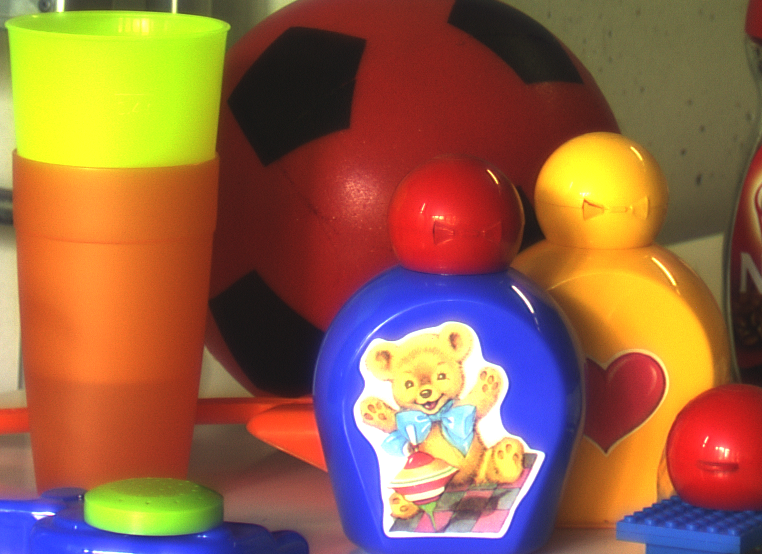
\includegraphics[width=0.45\textwidth]{images/img_all_channels.png} 
  }
  \subfigure[Extracted red channel]{
    \label{subfig:imgredchannel}
    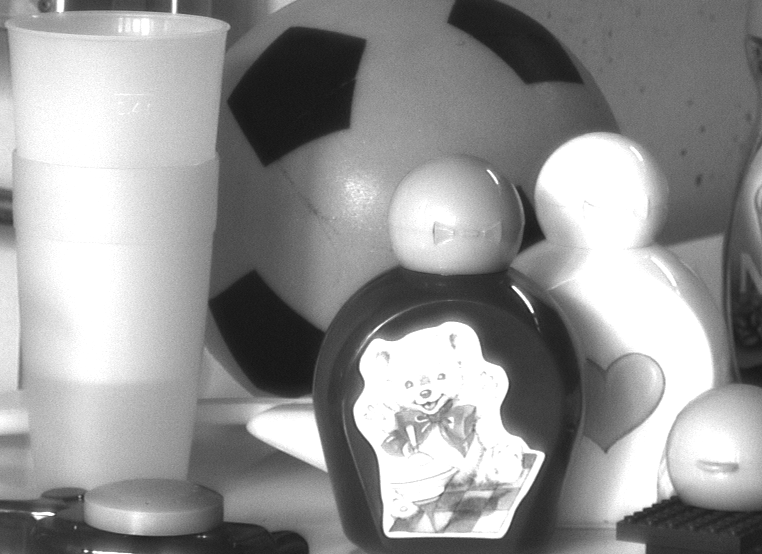
\includegraphics[width=0.45\textwidth]{images/img_red.png} 
  }
  \subfigure[Computed LISO map]{
    \label{subfig:lisomapred}
    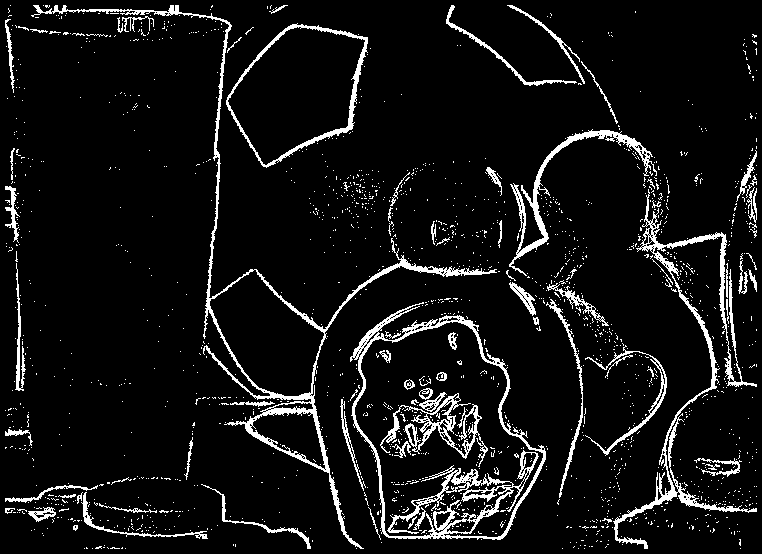
\includegraphics[width=0.8\textwidth]{images/liso_map_red.png} 
  }
  \caption[Example for a LISO map]{Example for a LISO map. \autoref{subfig:imgallchannels} shows the original image. In \autoref{subfig:imgredchannel} only the red channel is shown, which is used by the algorithm to generate the binary LISO map for the particular channel. The LISO map is shown in \autoref{subfig:lisomapred}. Note that most of the points in the LISO set lie around edges in the image.}
  \label{fig:lisomap}
\end{figure}
All in all, six features have to be computed:
\begin{itemize}
	\item error function value $E(R)$,
	\item gradient magnitude $\left|\mathrm{grad}(R)\right| = \sqrt{R_x^2+R_y^2}$\ ,
	\item normalized second derivative in gradient direction $\lambda = \frac{R_{gg}}{R_g^2}$, where $R_g$ and $R_{gg}$ are the first and second order partial derivatives in gradient direction,
	\item total mass $m_0 = \sum\limits_{(x,y)\in N_5} b(x,y)$, where $N_5$ denotes a $(5 \times 5)$ pixels neighborhood window,
	\item centroid $m_1$ and
	\item radius of gyration $m_2$.
\end{itemize}

For the training of the Bayes classifier, a set of training images is compiled by using either linear real-world or linear synthetic images and then applying different gamma curves with $\gamma \in [0.2; 0.6]$. 

As seen before, gamma curves are horizontal lines in $Q$-$R$ space, and so all points in $S_\text{LISO}$ are classified into $S_\text{LPIP}$ and $S_\text{non-LPIP}$ by the following criterion.
\begin{equation}
	(x,y) \in 
	\begin{cases}
	  S_\text{LPIP}				&\text{if} \ \ \left|Q(x,y) - \gamma\right| \leq 0.1 \\
	  S_\text{non-LPIP}		&\text{else}
	\end{cases}
	\label{eq:lpipclassification}
\end{equation}
Hence, all points in $S_\text{LPIP}$ have a $Q$ value close to $\gamma$. 

Let $c \in \left\{S_\text{LPIP}, S_\text{non-LPIP}\right\}$. Then $P(c) = \frac{\left|c\right|}{\left|S_\text{LISO}\right|}$, where $\left|\cdot\right|$ denotes the number of elements in a class. Therefore, $P(c)$ is the ratio of points belonging the the class $c$. The a-posterior probability of a LISO being a LPIP is then given by
\begin{equation}
	P(S_{LPIP}| \vec{f}) = 
	\frac{P(\vec{f}|S_\text{LPIP}) \cdot P(S_\text{LPIP})}{P(\vec{f}|S_\text{LPIP}) \cdot P(S_\text{LPIP}) + P(\vec{f}|S_\text{non-LPIP}) \cdot P(S_\text{non-LPIP})} \enspace ,
	\label{eq:aposterior}
\end{equation}
where $\vec{f} = [f_1, ..., f_6]$ is the six-dimensional feature vector containing the computed feature values. Let $h(c, i, v)$ the ratio of elements belonging to the respective bin for the feature value $v$ in the histogram of the $i$'th feature of the class $c$ over the entire number of elements in $c$. $P(\vec{f}|c)$ is then given by
\begin{equation}
	P(\vec{f}|c) = \prod\limits_{i=1}^{6} \frac{h(S_\text{LPIP}, i, f_i)}{h(S_\text{LPIP}, i, f_i) + h(S_\text{non-LPIP}, i, f_i)} \enspace .
	\label{eq:featureratios}
\end{equation}

The conditional probability function $P(S_\text{LPIP}| \vec{f})$ from \autoref{eq:aposterior} is used as a weighting function for the points in $S_\text{LISO}$, when it comes to the actual CRF estimation. The weighted \hbox{$Q$-$R$} histogram is also referred to as \emph{CRF signature} in Ng's subsequent publications \cite{ng_wifs09_1} and \cite{ng_wifs09_2}.


\clearpage

\subsubsection{CRF Estimation}
\label{subsubsec:CRFestimation}
As presented in \autoref{subsec:geoinvtheory}, the CRF estimation method is based on the GGCM model. Due to the tradeoff between modeling power and computational complexity, a first order GGCM \hbox{($n = 1$)} is used. Hence, the coefficient vector $\vec{\alpha} = \left[\alpha_0, \alpha_1\right]$ is only two-dimensional. Nevertheless, the model exhibits good fit to real-world CRFs in comparison to a purely polynomial model. 

Let $N = |S_\text{LISO}|$ and $Q_n$, $R_n$ and $\vec{f}_n$ the $Q$- and $R$-value and feature vector of the $n$-th element in $S_\text{LISO}$. The best possible coefficient vector $\vec{\alpha}^*$ can be determined by minimizing the objective function
\begin{equation}
	\vec{\alpha}^* = \mathrm{argmin} \ \sum\limits_{i = 1}^{N}{ \frac{P(S_{LPIP}| \vec{f}_i)}{P(R_i)} \ \left|Q_i - \widetilde{Q}(R_i,\vec{\alpha})\right|^2 } \enspace .
	\label{eq:objectivefunction}
\end{equation}
$P(R)$ is the ratio of points with this particular intensity value over all points in $S_\text{LISO}$. It is utilized to overcome polarization effects during the optimization, if the distribution of $R$ is unbalanced in the image. Given an inverse CRF $g_{\vec{\alpha}}$, where $\vec{\alpha}$ is the coefficient vector for GGCM, $\widetilde{Q}$ determines the $Q$-value corresponding to $R$,
\begin{equation}
	\widetilde{Q}(R, \vec{\alpha}) = \frac{g_{\vec{\alpha}}'(R)}{1 + g_{\vec{\alpha}}''(R) \cdot R} \enspace .
	\label{eq:Qtilde}
\end{equation}

\vspace{1cm}

\subsubsection{Refinement}
\label{subsubsec:refinement}

Ng et \hbox{al.} propose an additional refinement by a calibration, when linearizing $Q(R)$ with respect to the differential change of the gamma curve parameter $\gamma$:
\begin{equation}
	\overline{Q}(R) = \frac{\sqrt{3}}{\sqrt{3} - 1} \left(1 - \sqrt{1 - \frac{1}{2 \cdot Q(R)+1}}\ \right) \enspace .
	\label{eq:calibration}
\end{equation}
Note that every $Q$-value has to be computed this way for the refinement to take effect. 